\documentclass[journal,twoside,web]{ieeecolor}
\usepackage{jsen}
\usepackage{cite}
\usepackage{amsmath,amssymb,amsfonts}
\usepackage{algorithmic}
\usepackage{graphicx}
\usepackage{textcomp}
\usepackage{wrapfig}
\usepackage{biblatex}
\addbibresource{covid.bib}
\def\BibTeX{{\rm B\kern-.05em{\sc i\kern-.025em b}\kern-.08em
    T\kern-.1667em\lower.7ex\hbox{E}\kern-.125emX}}
\markboth{Spring 2020}
{Author \MakeLowercase{\textit{et al.}}: SARS-CoV-2 and Healthy Diet (March 2021)}
\begin{document}
\title{SARS-CoV-2 and Healthy Diet}
\author{Rajinder Singh, Big Data Analytics, Masters of Computer Science,loo157049@student.lyit.ie,  Letterkenny Institute of Technology

\thank{Under the supervision of Dr. Shagufta Henna, Letterkenny Institute of Technology, Letterkenny, CO. Donegal}
}

\IEEEtitleabstractindextext{\begin{wrapfigure}[12]{r}{3in}%

\includegraphics[width=3in]{fig1.jpeg}%
\end{wrapfigure}%
\begin{abstract}
SARS-CoV-2 is the new strain of highly contagious coronavirus that is spreading all over the world at an exponential rate. It has flu-like symptoms and attacks humans' respiratory systems. Scientists are researching the genome of this virus to determine its behavior and the possibilities of mutations. This paper is an attempt to determine whether there is a correlation between the type of food we consume and the mortality rate of countries. Moreover, we will compare the obesity and undernourishment data of the countries with covid infections to unravel the relation between them. Using the machine learning algorithms, we will analyze the data and try to cluster it to predict the deaths due to covid-19. The study would serve as a foundation of further research and each aspect can be studied in detail.
\end{abstract}

\begin{IEEEkeywords}
Covid-19, Healthy Diet, Big Data Analytics, Obesity, Undernourishment, Fatality rate, K-means, Linear Regression, Coronavirus, Cambodia, United States, Animal Products
\end{IEEEkeywords}}

\maketitle
\section{Introduction}
\label{sec:introduction}
\IEEEPARstart{T}{he} world is amid a pandemic. Many countries are under full lockdown and some are in partial lockdown. The economies are struggling to survive while unemployment \cite{blustein2020unemployment} is all-time high. Developing and poor countries \cite{chin2020stability} are high on the hunger index and mental health becomes a most serious issue than the virus itself. The pandemic showing the mirror to mankind and bring the possibility to introspect where we are heading to. Sars Covid 2 \cite{chin2020stability}, commonly known as Covid-19 is a highly contagious disease that spreads in almost every part of the world. Currently, we have multiple vaccinations which are being given to people worldwide to eradicate the disease. 

Almost after a year of fighting the pandemic, we have sufficient data to incorporate Machine learning and Artificial Intelligence to do research on the virus. It is observed that the rate of infection and mortality is different in different parts of the world \cite{meo2020biological}. There could be many factors leading to this inequality such as high population density, government strategies to curb covid, weather, immune systems, earlier vaccinations, healthcare, or diet.

In this paper, we are going to focus on diet and its effect on the virus. The database \cite{noauthor_food_nodate} will have statistics for the intake of animal fats, vegetable fats, vegetable protein, animal protein, milk and dairy product consumption, and many other parameters for each country. Other than this, we will compare the undernourished and obesity data with the covid 19 data \cite{noauthor_covid-19_nodate} among the countries to determine any correlation among these parameters. We will attempt to do clustering of the given data with Kmeans clustering algorithm \cite{likas2003global} and observe the output. We will then apply Linear regression and Random forest regression on the data to predict the mortality rate with the help of the selected features. In the end we will represent results with the help of visualizations and interpret the findings. This paper follows the Big Data Analytics pipeline model and every stage will be discussed in the following sections.

\section{Dataset Overview}
This project incorporates different datasets collected from multiple organisations and merged to perform analytics. It holds the Covid-19 mortality database, countrywide undernourished, and obesity datasets. Also, the data for various food group supply quantities, nutrition values are obtained from FAO (Food and Agriculture Organisation) of the UN \cite{noauthor_food_nodate}. All these databases are blended to form a single dataset which provides the parameters discussed below. All data is available in the public domain and is available from the given links in the references.

\subsubsection{Covid Dataset}
The Covid-19 dataset is a day-wise distribution of covid 19 confirmed, death, and active cases among the countries. The data is provided by "Johns Hopkins Center for Systems Science and Engineering CSSE website" \cite{noauthor_covid-19_nodate}. In this dataset we have the following significant parameters:


\begin{itemize}
    \item Observation Date - Date of the observation in MM/DD/YYYY
    \item Country/Region - Country name
    \item Confirmed - Number of cases confirmed till date
    \item Deaths - Number of deaths encountered till that date
    \item Recovered - Number of recoveries till that date
\end{itemize}
We will need Country, confirmed, deaths, and Recovered cases data from this dataset which we will merge with other available data sets as discussed further.

\subsubsection{Food and Nutrition Data-set}
This dataset includes food intake in all the countries worldwide. It also incorporates obesity and undernourished counts in addition to the total population in that country. The food intake is measured in kilograms and all the columns are represented as percentages except population. The dataset includes columns like Animal fats intake, vegetable products, meat, cereals, eggs, seafood, and many others. These parameters act as the potential candidates of the features for ML algorithms.

\section{Data Processing and Exploration}
The main focus of the first stage is to refine and cast the data to visualize it. The covid-19 dataset needs to be transformed into percentages. For instance, the percentage of confirmed cases in a country out of the total confirmed cases. In this way, the size of the dataset will be reduced to the number of countries only and we will have more comprehensive data. We have two datasets, one with covid 19 data and another one with nutrition data as discussed earlier. Now, we need to join both the datasets based on the country name. After joining the databases \cite{drabas2017learning}, it will look like Figure 1.
\begin{figure}[!t]
\centerline{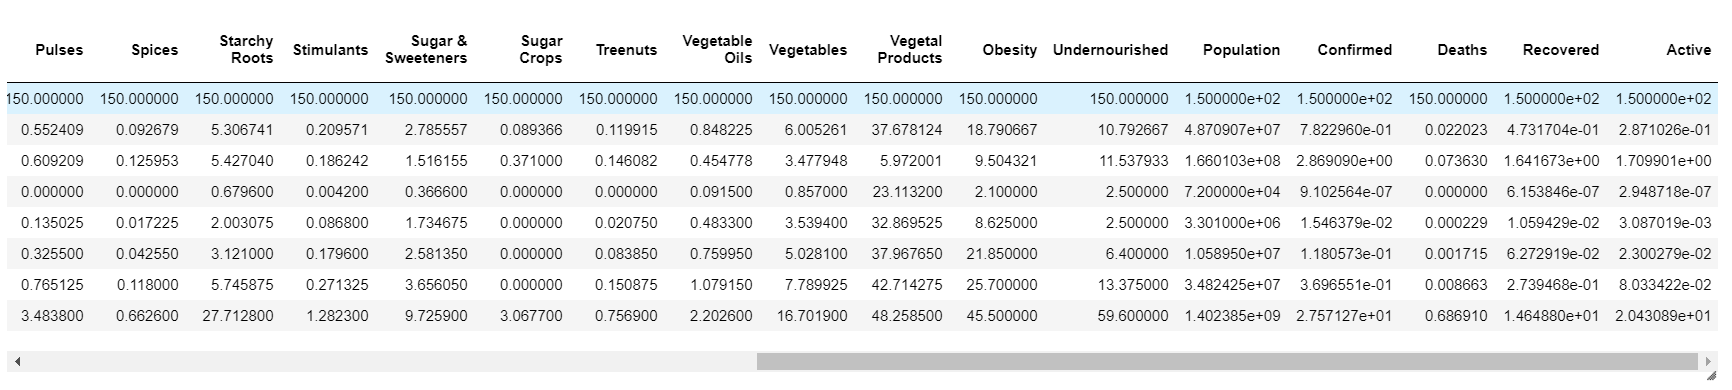
\includegraphics[width=\columnwidth]{profig0.png}}
\caption{Dataset after joining operation.
Nutrition data is merged with corresponding covid metrics for every country}
\label{fig1}
\end{figure}
Once the datasets are joined, we can now remove the irregularities such as NULL or NAN values in the dataset. Also, the datatype of Undernourished and Obesity must be cast into double datatypes for further calculations. We will summarize function to calculate the mean, variance count, and other statistics parameters to have a better understanding of the data. At the end of this section, our database will be
\begin{itemize}
    \item without null values
    \item all numeric columns of double type 
    \item each numeric cell will represent the percentage of the metric.
\end{itemize}
After removing the null values, the dataset now can be fancied using pie charts and scattered charts \cite{keim2013big} as shown in the Figure 2.
\begin{figure}[!t]
\centerline{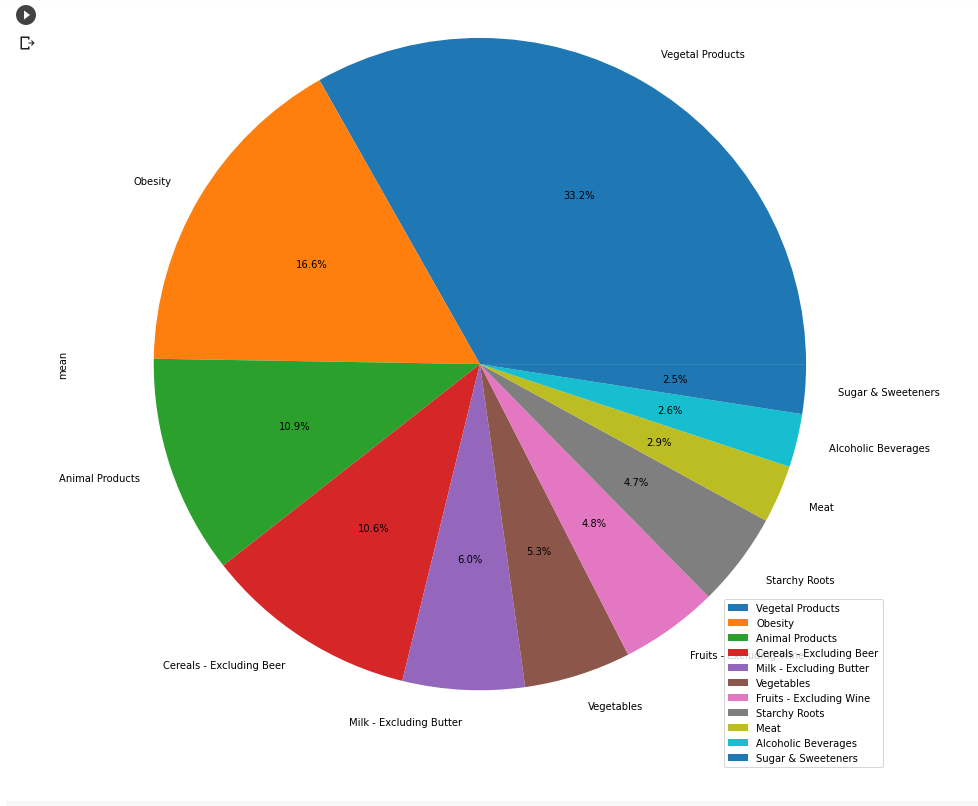
\includegraphics[width=\columnwidth]{profig1.png}}
\caption{Type of food products and their consumptions.}
\label{fig1}
\end{figure}

Figure 2 Clearly shows that vegetal products are the most consumed products followed by animal products and cereals. This chart will be used in the visualizations to compare it with other significant metrics in further sections.

\begin{figure}[!t]
\centerline{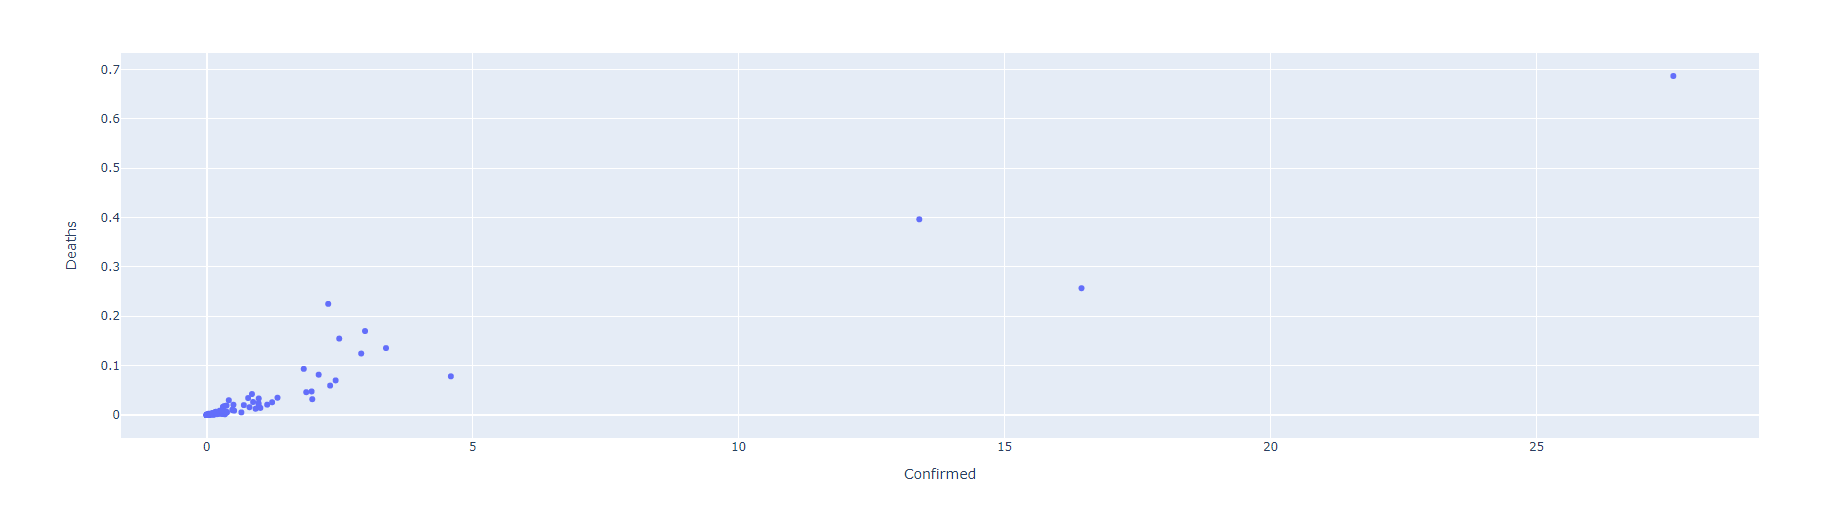
\includegraphics[width=\columnwidth]{progif2.png}}
\caption{This graph gives a sense of repartition of countries in function of their covid deaths and confirmed case. Extremes can be easily spotted.}
\label{fig1}
\end{figure}

Fig. 3.  Shows the scatter plot of covid 19 deaths in all the countries. One can easily observe the extremes in the charts to determine which country is highly affected by a coronavirus and which is least.

\section{Big data architecture and tools}
The project is set up and deployed on the virtual machine using Databricks. It has installed multiple libraries installed such as NumPy, pandas, seaborn, matplotlib, pyspark, spark magic, plotly, Mlib, and other required libraries \cite{drabas2017learning}.

\begin{figure}[!t]
\centerline{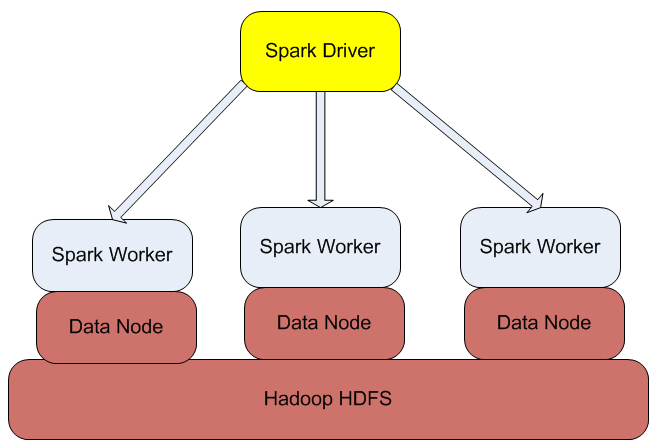
\includegraphics[width=\columnwidth]{profig3.png}}
\caption{Big Data Architecture with Spark and Hadoop}
\label{fig1}
\end{figure}

The project mainly focused on data processing and handling with the spark data frame. The programming interface used is Pyspark and Jupyter notebook as it provides more flexibility and mobility of code. For visualizations, the project mainly relies on the pandas' data frame and plotly \cite{sievert2020interactive} as they provide more features and compatibility than others. The entire project runs in the context of Spark especially the machine learning algorithms and pipeline stages of the process such as scaling, featuring, and clustering.
\label{sec:guidelines}

\subsection{Data Pipeline}
A data pipeline architecture is more of a layered architecture in which the output of one step feeds as input to the next step until unless it reaches its destination.
\subsubsection{Data Source}
We can load data from multiple sources such as RDBMS, APIs, MongoDb, Cloud sources (Amazon S3 Bucket), FTP, Hadoop, and many more. Once the data is retrieved, one must adhere to security measures and obey practices for performance and consistency.
\subsubsection{Extraction}
Any masking or encrypting of unique elements such as zip codes in an address field or any categorical values can be done by data extraction. It also helps in the GDPR alliance like eliminating the emails or personal information of a person from the dataset by masking or using any other technique.

\subsubsection{Joins}
Joins are a very common step in the pipeline. It is used when multiple data from different sources need to be joined into one to reduce the dataset size and complexity.

\subsubsection{Standardization}
It is often required that all the measurable columns must be of the same units or dimensions to perform the operations. A similar requirement comes in our database, where we had percentage data of food data but covid data was commutative. So, we converted the covid data into percentage data so that it can be joined together to perform further transformations.

\subsubsection{Correction}
Correction is the scenario where we remove or correct the values in the columns of the data type of the column which is not recorded correctly. For example, removing null and NaN or converting the Undernourished column from string to numerical and vice versa.

\subsubsection{Feature Engineering}
When the dataset is complex and big enough that one cannot decide which features or columns are significant and which are useless, feature engineering comes into place. 

\subsection{Pearson Correlation}
The Pearson correlation \cite{benesty2009pearson} is used to find the strength of the linear association between any two variables. It is denoted by r. In other words, the Pearson correlation tries to plot the line between the two variables and r denotes the value far from that linear line. If the points lie on or close to the line, the relation is highly linear and vice versa.
In our database, we will attempt to find a linear relationship between health conditions such as obesity and undernourishment against covid metrics.
After that, we will plot a heat map of r values obtained and observe the results as in the figure 5.

\begin{figure}[!t]
\centerline{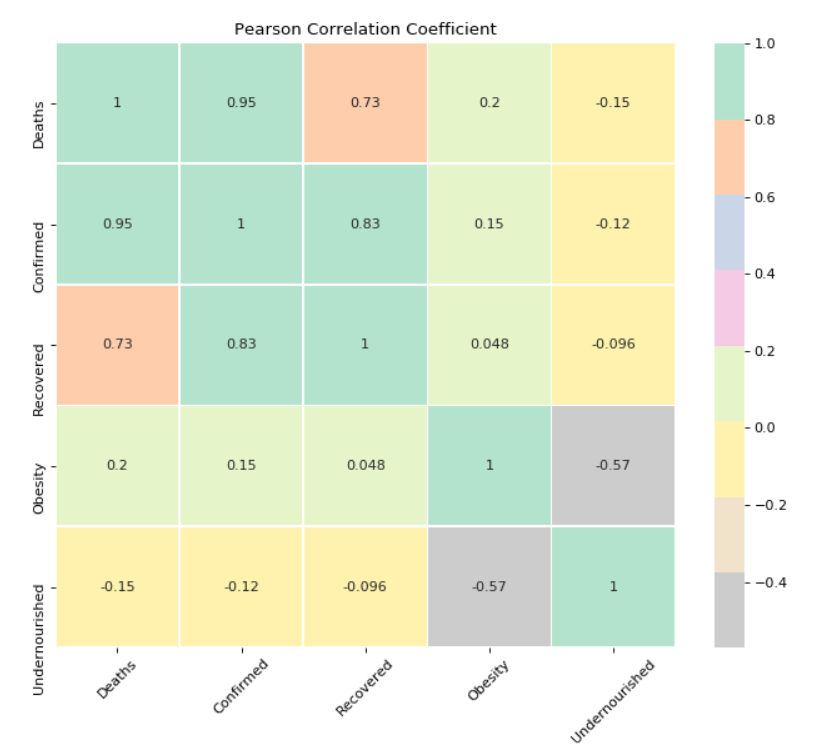
\includegraphics[width=\columnwidth]{profig4.png}}
\caption{Heatmap between Covid metrics and health conditions}
\label{fig1}
\end{figure}

We can observe that obesity has a significant correlation with mortality rate than recovery. On the other hand, undernourishment has a stronger correlation with the recovery rate.
\subsection{Features Engineering}
Two main functions of feature engineering \cite{drabas2017learning} are to provide compatible input to the Machine learning algorithms and to improve their performance. It is achieved by helping the program to choose the more significant features which help in better predictions and identify features which mislead the algorithms and cause errors.

Unsupervised algorithms \cite{celebi2016unsupervised} make deductions based on input vectors only without referring to named labels. K means first selects the centroids \cite{likas2003global} randomly and makes iterative computations on data to adjust their positions accurately. The breaking point of the process is:
\begin{itemize}
    \item when clusters' position is stabilized or no more optimization needed
    \item when the number of iterations has been achieved.
\end{itemize}

\subsection{Linear Regression}
The most basic and commonly used predictive analysis is Linear Regression. The basic idea behind the linear regression \cite{montgomery2021introduction} is to
\begin{itemize}
    \item determine if predictor variables are capable to predict dependent variable values
    \item identify the variables that are more significant in predicting the dependent variable.
\end{itemize}
It is used to find the relationship between one dependent variable with the one or more independent variables and is defined by the formula y = m*x + c, where y is the dependant variable, c is the constant, b is the regression coefficient and x is the score on the independent variable.

In our case, the independent variables are Alcoholic Beverages, Seafood, Animal fats, Animal Products, Aquatic Products, Other, Milk - Excluding Butter, Cereals - Excluding Beer, Active, Eggs, Fish, Vegetal Products, Meat, Miscellaneous, Offals, Oilcrops, Pulses, Starchy Roots, Stimulants, Sugar & Sweeteners, Sugar Crops, Treenuts, Vegetable Oils, Vegetables, Obesity, Undernourished, Confirmed, Fruits - Excluding Wine, Recovered while dependent variable is Deaths 

Root Mean Square Error (RMSE) is the standard deviation of prediction errors. It tells us the data concentration around the line of best fit. After applying Linear Regression, we calculated the RMSE \cite{chai2014root} value to find the efficacy of the model.  In our case, the RMSE is 0.54 which is not a very great value. It describes that there is some correlation between the features and labels but it is not strong and concrete. We need to refine the features and have a future scope of research.


\subsection{Random Forest Regression}
Random forest is a Supervised Learning algorithm \cite{liaw2002classification} that uses an aggregate training method for ranking and regression.
It functions by forming a plenitude of decision trees at training time and outputting the class that is the mean prediction of the singular tree. It consolidates the outcomes of multiple predictions which aggregates many decision trees, with some helpful modifications.
In predicting the mortality rate, random forest proved to be way better than the linear regression. After training and fitting the model, the prediction is accurate up to 76% which is 20% better than the linear regression. 
\subsubsection{Advantages of Random Forest}
\begin{itemize}
    \item It is compatible with most of the datasets and gives high accuracy rate than other regression algorithms.
    \item it works efficiently with heavy datasets
    \item it provide the list of most important features in the regression which one can analyse and decide to remove if necessary to experiment with less significant features.
\end{itemize}

Despite of some benefits, Random forest comes with a disadvantage where it proved biased towards the attributes which has more levels. So, it is not the case that Random forest will give accurate results all the time.

\section{Results}
After performing all the pipeline steps, we can now interpret the results. We have final visualizations, predictions, RMSE values of ML regression models, and clustering data results. Let find out what we learn so far from our findings.

Random Forest regression provides the top important features on which the mortality rate depends. Other than deaths, active, recovered are the important factors as well. When talking about diet indicators, Offlas, Alcoholic Beverages,  Pulses, Oilcrops, and Obesity are among the top 10 important features which help in predicting the mortality rate of covid cases as shown in Fig.

By Pearson Coefficient Regression, we observed that Obesity has a significant correlation with the mortality rate than recovery and on the other hand, undernourishment has a correlation with recoveries.

\begin{figure}[!t]
\centerline{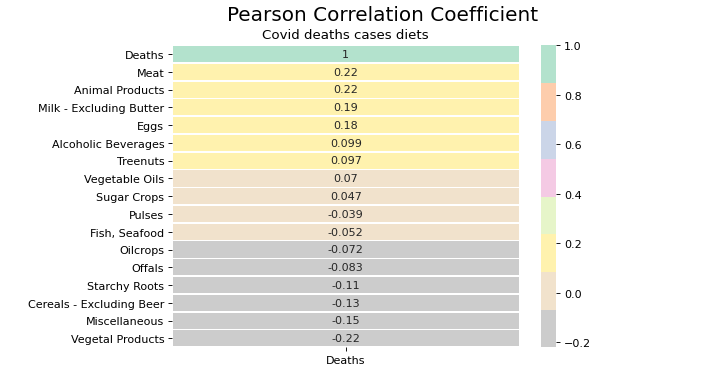
\includegraphics[width=\columnwidth]{profig11.png}}
\caption{Pearson Correlation Coefficient}
\label{fig1}
\end{figure}

We can infer that obese patients are more likely to die of covid than anyone else and undernourished has not to impact on covid deaths. These results are based on the dataset available and there may be multiple reasons which can cause the mortality rate high other than just diet.

\begin{figure}[!t]
\centerline{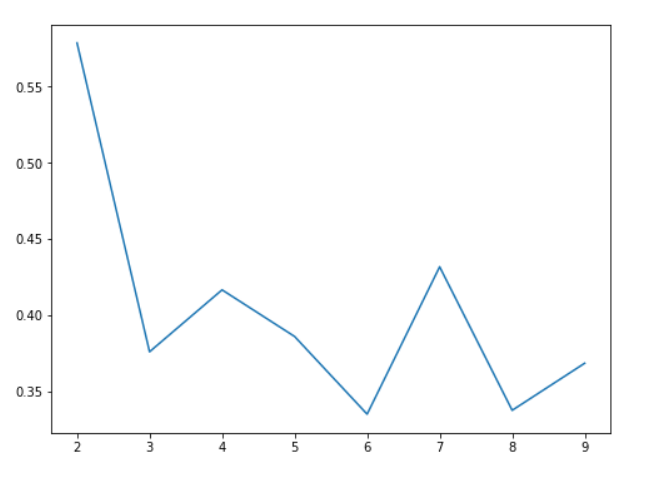
\includegraphics[width=\columnwidth]{profig5.png}}
\caption{Silhouette score of Kmeans clustering}
\label{fig1}
\end{figure}

\subsection{United States with highest mortality rate}
It is interesting to see that the US has a 37.3% obesity rate, which could be a partial reason for having a high death rate due to Coivd-19.
\begin{figure}[!t]
\centerline{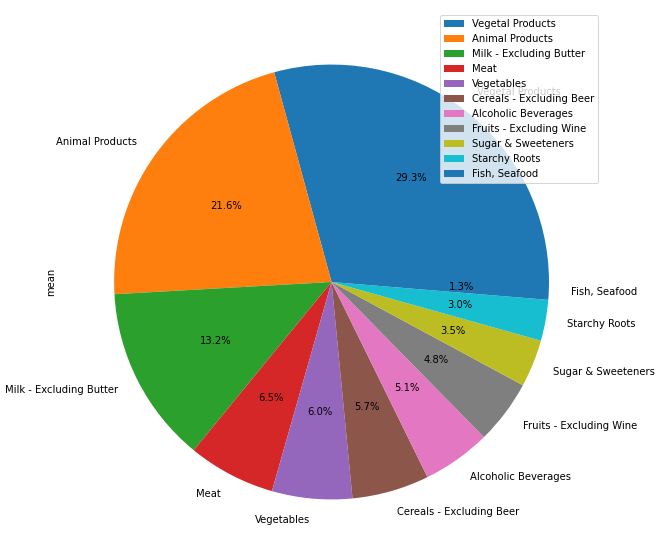
\includegraphics[width=\columnwidth]{profig7.png}}
\caption{United States diet metrics distribution}
\label{fig1}
\end{figure}
The pie chart above, clearly depicts that the United States consumes animal products more than the average world's consumption. Even they are consuming more than the average obese diet.

\subsection{United States with highest confirmed cases}
The United States again with one of the most confirmed cases in the world.
Again, obesity is all-time high with 35.3% which is way more than the average.
The pie chart in figure 8 shows that the confirmed also shares the same statistics as we have in the mortality rate. The US being highest in both the mortality and confirmed cases depicts that their dietary habits have a significant effect on the rising infections.


\subsection{Vanuatu : less confirmed cases in relation to its population}
Vanuatu has a whole new different story to tell. It has a high obesity rate of 23.5% but the mortality rate and confirmed covid cases are way lower than the rest of the world. There must be multiple reasons behind it. As we are dealing with diet, we will try to figure out what makes them stand out different from the rest of the world with the help of the figure below.

\begin{figure}[!t]
\centerline{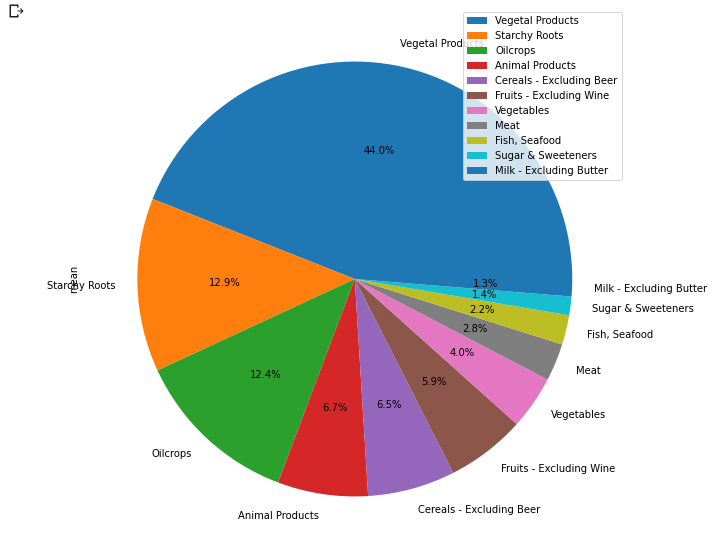
\includegraphics[width=\columnwidth]{profig9.png}}
\caption{Vanuatu diet metrics distribution}
\label{fig1}
\end{figure}

Vanuatu's people consume way less meat or animal products when compared to the US. Also, there is a high intake of starchy roots and Oilcrops.

\subsection{Cambodia : with the lowest mortality rate in relation to its population}
Cambodia is a country with a very low obesity rate and the interesting fact is that they have the high undernourished one. For most of the food, the population of Cambodia consumes starchy roots and cereals (excluding beers). Being high on undernourishment raises the possibility that Undernourishment does not affect Covid mortality rates \cite{neak2021cambodia}. This could be an open domain for whole new research for further studies.

\begin{figure}[!t]
\centerline{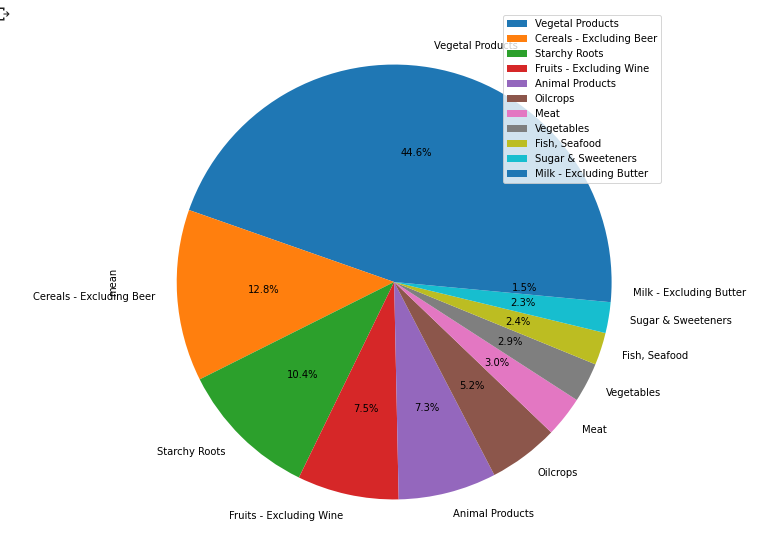
\includegraphics[width=\columnwidth]{profig10.png}}
\caption{Cambodia diet metrics distribution}
\label{fig1}
\end{figure}

\section{Conclusion}
In conclusion, now we have executed ML algorithms and studied the pie charts above, we can deduce some key points. Firstly, the Pearson Correlation Coefficient plot shows that obesity has a stronger correlation with covid deaths than any other factor and undernourishment has a significant correlation with the recovery rates altogether. Furthermore, other than animal products, alcoholic beverages could also be the reason for the high fatality rate in the United States. But we do not have concrete outcomes to confirm this which creates the scope of research.

The important point to be noticed that the outcomes only rely on the dataset available. This is just an attempt to study the virus from a new perspective. But most of the established factors such as age, sex, underline health conditions, and previous vaccine history is ignored in this project. There is ample scope to include nutrition elements in the ongoing researches to better predict the future of the virus in further studies.

Cambodia seems to be the winner here but we cannot deny the fact that the effective government strategy and lockdowns helped to curb the virus in the country thus this could be the dominating factor for the low mortality and infection rate there.

We also observed that Linear Regression did not go well with the covid database and gave the efficacy of 54% while predicting deaths. Manual clustering also didn't go well but K-means attempted to segregate the data into clusters. Random forest did pretty well and gave us the most important factors which help to determine the fatality rate.

We had a limited dataset which mainly focused on diet and covid metrics. There could be many other factors that can drive the mortality and infection rates in the countries. In further studies and researches, we can consider these top nutrients factors concluded to increase the efficacy of the trained models, and predictions can improve their efficacy. 

\printbibliography

\end{document}
